\begin{figure}[t]
\centering
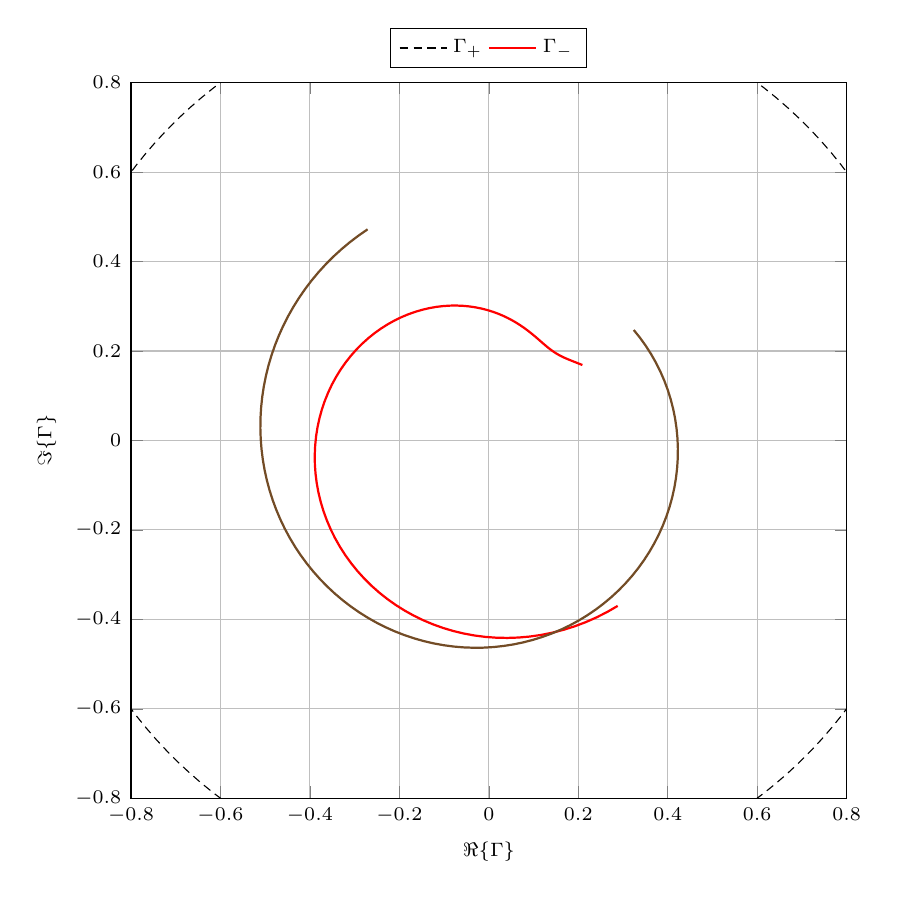
\begin{tikzpicture}
\begin{axis}[
width=\columnwidth,
height=0.88\columnwidth,
axis equal image,
xmin=-0.8,xmax=0.8,
ymin=-0.8,ymax=0.8,
xlabel={$\Re\{\Gamma\}$},
ylabel={$\Im\{\Gamma\}$},
grid=both,
tick label style={font=\scriptsize},
label style={font=\scriptsize},
legend style={font=\scriptsize,at={(0.5,1.02)},anchor=south,legend columns=2},
]
\addplot[densely dashed,domain=0:360,samples=181] ({cos(x)},{sin(x)});
\addplot+[thick,mark=none] table[x=gpr,y=gpi] {
f gpr gpi gmr gmi
9.000 0.28813171 -0.36993592 0.32399824 0.24698925
9.025 0.26462696 -0.38352928 0.33789603 0.22969837
9.050 0.24066858 -0.39567333 0.35083576 0.21169080
9.075 0.21633418 -0.40637127 0.36278394 0.19302143
9.100 0.19169920 -0.41562870 0.37371038 0.17374634
9.125 0.16683704 -0.42345344 0.38358817 0.15392263
9.150 0.14181926 -0.42985543 0.39239365 0.13360824
9.175 0.11671574 -0.43484663 0.40010639 0.11286175
9.200 0.09159479 -0.43844092 0.40670915 0.09174222
9.225 0.06652333 -0.44065416 0.41218783 0.07030908
9.250 0.04156694 -0.44150413 0.41653144 0.04862190
9.275 0.01678998 -0.44101055 0.41973208 0.02674036
9.300 -0.00774438 -0.43919515 0.42178485 0.00472399
9.325 -0.03197409 -0.43608172 0.42268785 -0.01736786
9.350 -0.05583823 -0.43169613 0.42244212 -0.03947620
9.375 -0.07927704 -0.42606645 0.42105160 -0.06154252
9.400 -0.10223192 -0.41922298 0.41852305 -0.08350888
9.425 -0.12464550 -0.41119833 0.41486604 -0.10531809
9.450 -0.14646172 -0.40202749 0.41009286 -0.12691379
9.475 -0.16762596 -0.39174788 0.40421847 -0.14824055
9.500 -0.18808511 -0.38039938 0.39726046 -0.16924403
9.525 -0.20778776 -0.36802438 0.38923893 -0.18987106
9.550 -0.22668431 -0.35466781 0.38017647 -0.21006975
9.575 -0.24472717 -0.34037711 0.37009806 -0.22978961
9.600 -0.26187092 -0.32520222 0.35903098 -0.24898164
9.625 -0.27807250 -0.30919558 0.34700474 -0.26759843
9.650 -0.29329142 -0.29241202 0.33405099 -0.28559426
9.675 -0.30748992 -0.27490872 0.32020341 -0.30292518
9.700 -0.32063322 -0.25674508 0.30549763 -0.31954908
9.725 -0.33268968 -0.23798263 0.28997113 -0.33542582
9.750 -0.34363099 -0.21868485 0.27366311 -0.35051722
9.775 -0.35343240 -0.19891701 0.25661442 -0.36478722
9.800 -0.36207284 -0.17874600 0.23886744 -0.37820188
9.825 -0.36953513 -0.15824011 0.22046594 -0.39072944
9.850 -0.37580611 -0.13746877 0.20145502 -0.40234041
9.875 -0.38087679 -0.11650233 0.18188094 -0.41300755
9.900 -0.38474245 -0.09541181 0.16179108 -0.42270600
9.925 -0.38740276 -0.07426857 0.14123372 -0.43141322
9.950 -0.38886183 -0.05314404 0.12025805 -0.43910907
9.975 -0.38912829 -0.03210944 0.09891394 -0.44577582
10.000 -0.38821532 -0.01123541 0.07725190 -0.45139819
10.025 -0.38614061 0.00940829 0.05532295 -0.45596332
10.050 -0.38292640 0.02975309 0.03317848 -0.45946080
10.075 -0.37859939 0.04973196 0.01087016 -0.46188269
10.100 -0.37319066 0.06927977 -0.01155016 -0.46322349
10.125 -0.36673562 0.08833356 -0.03403060 -0.46348014
10.150 -0.35927380 0.10683292 -0.05651933 -0.46265204
10.175 -0.35084874 0.12472028 -0.07896468 -0.46074097
10.200 -0.34150779 0.14194126 -0.10131529 -0.45775114
10.225 -0.33130193 0.15844490 -0.12352013 -0.45368911
10.250 -0.32028545 0.17418403 -0.14552871 -0.44856380
10.275 -0.30851576 0.18911548 -0.16729109 -0.44238643
10.300 -0.29605308 0.20320036 -0.18875805 -0.43517051
10.325 -0.28296012 0.21640431 -0.20988115 -0.42693175
10.350 -0.26930173 0.22869765 -0.23061284 -0.41768806
10.375 -0.25514457 0.24005566 -0.25090655 -0.40745950
10.400 -0.24055674 0.25045865 -0.27071679 -0.39626818
10.425 -0.22560734 0.25989217 -0.28999922 -0.38413825
10.450 -0.21036612 0.26834707 -0.30871075 -0.37109581
10.475 -0.19490302 0.27581957 -0.32680963 -0.35716885
10.500 -0.17928775 0.28231135 -0.34425551 -0.34238720
10.525 -0.16358934 0.28782949 -0.36100951 -0.32678243
10.550 -0.14787570 0.29238649 -0.37703432 -0.31038779
10.575 -0.13221316 0.29600019 -0.39229424 -0.29323816
10.600 -0.11666600 0.29869366 -0.40675524 -0.27536990
10.625 -0.10129602 0.30049504 -0.42038507 -0.25682085
10.650 -0.08616207 0.30143741 -0.43315323 -0.23763019
10.675 -0.07131963 0.30155851 -0.44503110 -0.21783839
10.700 -0.05682034 0.30090050 -0.45599196 -0.19748711
10.725 -0.04271164 0.29950965 -0.46601102 -0.17661909
10.750 -0.02903629 0.29743601 -0.47506547 -0.15527812
10.775 -0.01583208 0.29473300 -0.48313453 -0.13350888
10.800 -0.00313142 0.29145698 -0.49019946 -0.11135691
10.825 0.00903900 0.28766684 -0.49624362 -0.08886846
10.850 0.02065842 0.28342341 -0.50125246 -0.06609047
10.875 0.03171238 0.27878899 -0.50521356 -0.04307038
10.900 0.04219283 0.27382674 -0.50811665 -0.01985613
10.925 0.05209838 0.26860012 -0.50995361 0.00350400
10.950 0.06143438 0.26317216 -0.51071849 0.02696145
10.975 0.07021304 0.25760489 -0.51040751 0.05046748
11.000 0.07845338 0.25195860 -0.50901904 0.07397330
11.025 0.08618127 0.24629114 -0.50655364 0.09743011
11.050 0.09342928 0.24065718 -0.50301400 0.12078922
11.075 0.10023651 0.23510747 -0.49840498 0.14400216
11.100 0.10664839 0.22968807 -0.49273354 0.16702072
11.125 0.11271636 0.22443962 -0.48600874 0.18979709
11.150 0.11849745 0.21939652 -0.47824175 0.21228391
11.175 0.12405389 0.21458622 -0.46944577 0.23443436
11.200 0.12945250 0.21002845 -0.45963605 0.25620227
11.225 0.13476411 0.20573445 -0.44882983 0.27754215
11.250 0.14006285 0.20170631 -0.43704634 0.29840932
11.275 0.14542536 0.19793620 -0.42430671 0.31875996
11.300 0.15092988 0.19440578 -0.41063401 0.33855123
11.325 0.15665535 0.19108549 -0.39605313 0.35774131
11.350 0.16268035 0.18793402 -0.38059077 0.37628950
11.375 0.16908194 0.18489766 -0.36427536 0.39415632
11.400 0.17593450 0.18190981 -0.34713696 0.41130357
11.425 0.18330840 0.17889045 -0.32920713 0.42769440
11.450 0.19126864 0.17574557 -0.31051882 0.44329329
11.475 0.19987335 0.17236665 -0.29110617 0.45806610
11.500 0.20917217 0.16863001 -0.27100428 0.47197985
};
\addplot+[thick,mark=none] table[x=gmr,y=gmi] {
f gpr gpi gmr gmi
9.000 0.28813171 -0.36993592 0.32399824 0.24698925
9.025 0.26462696 -0.38352928 0.33789603 0.22969837
9.050 0.24066858 -0.39567333 0.35083576 0.21169080
9.075 0.21633418 -0.40637127 0.36278394 0.19302143
9.100 0.19169920 -0.41562870 0.37371038 0.17374634
9.125 0.16683704 -0.42345344 0.38358817 0.15392263
9.150 0.14181926 -0.42985543 0.39239365 0.13360824
9.175 0.11671574 -0.43484663 0.40010639 0.11286175
9.200 0.09159479 -0.43844092 0.40670915 0.09174222
9.225 0.06652333 -0.44065416 0.41218783 0.07030908
9.250 0.04156694 -0.44150413 0.41653144 0.04862190
9.275 0.01678998 -0.44101055 0.41973208 0.02674036
9.300 -0.00774438 -0.43919515 0.42178485 0.00472399
9.325 -0.03197409 -0.43608172 0.42268785 -0.01736786
9.350 -0.05583823 -0.43169613 0.42244212 -0.03947620
9.375 -0.07927704 -0.42606645 0.42105160 -0.06154252
9.400 -0.10223192 -0.41922298 0.41852305 -0.08350888
9.425 -0.12464550 -0.41119833 0.41486604 -0.10531809
9.450 -0.14646172 -0.40202749 0.41009286 -0.12691379
9.475 -0.16762596 -0.39174788 0.40421847 -0.14824055
9.500 -0.18808511 -0.38039938 0.39726046 -0.16924403
9.525 -0.20778776 -0.36802438 0.38923893 -0.18987106
9.550 -0.22668431 -0.35466781 0.38017647 -0.21006975
9.575 -0.24472717 -0.34037711 0.37009806 -0.22978961
9.600 -0.26187092 -0.32520222 0.35903098 -0.24898164
9.625 -0.27807250 -0.30919558 0.34700474 -0.26759843
9.650 -0.29329142 -0.29241202 0.33405099 -0.28559426
9.675 -0.30748992 -0.27490872 0.32020341 -0.30292518
9.700 -0.32063322 -0.25674508 0.30549763 -0.31954908
9.725 -0.33268968 -0.23798263 0.28997113 -0.33542582
9.750 -0.34363099 -0.21868485 0.27366311 -0.35051722
9.775 -0.35343240 -0.19891701 0.25661442 -0.36478722
9.800 -0.36207284 -0.17874600 0.23886744 -0.37820188
9.825 -0.36953513 -0.15824011 0.22046594 -0.39072944
9.850 -0.37580611 -0.13746877 0.20145502 -0.40234041
9.875 -0.38087679 -0.11650233 0.18188094 -0.41300755
9.900 -0.38474245 -0.09541181 0.16179108 -0.42270600
9.925 -0.38740276 -0.07426857 0.14123372 -0.43141322
9.950 -0.38886183 -0.05314404 0.12025805 -0.43910907
9.975 -0.38912829 -0.03210944 0.09891394 -0.44577582
10.000 -0.38821532 -0.01123541 0.07725190 -0.45139819
10.025 -0.38614061 0.00940829 0.05532295 -0.45596332
10.050 -0.38292640 0.02975309 0.03317848 -0.45946080
10.075 -0.37859939 0.04973196 0.01087016 -0.46188269
10.100 -0.37319066 0.06927977 -0.01155016 -0.46322349
10.125 -0.36673562 0.08833356 -0.03403060 -0.46348014
10.150 -0.35927380 0.10683292 -0.05651933 -0.46265204
10.175 -0.35084874 0.12472028 -0.07896468 -0.46074097
10.200 -0.34150779 0.14194126 -0.10131529 -0.45775114
10.225 -0.33130193 0.15844490 -0.12352013 -0.45368911
10.250 -0.32028545 0.17418403 -0.14552871 -0.44856380
10.275 -0.30851576 0.18911548 -0.16729109 -0.44238643
10.300 -0.29605308 0.20320036 -0.18875805 -0.43517051
10.325 -0.28296012 0.21640431 -0.20988115 -0.42693175
10.350 -0.26930173 0.22869765 -0.23061284 -0.41768806
10.375 -0.25514457 0.24005566 -0.25090655 -0.40745950
10.400 -0.24055674 0.25045865 -0.27071679 -0.39626818
10.425 -0.22560734 0.25989217 -0.28999922 -0.38413825
10.450 -0.21036612 0.26834707 -0.30871075 -0.37109581
10.475 -0.19490302 0.27581957 -0.32680963 -0.35716885
10.500 -0.17928775 0.28231135 -0.34425551 -0.34238720
10.525 -0.16358934 0.28782949 -0.36100951 -0.32678243
10.550 -0.14787570 0.29238649 -0.37703432 -0.31038779
10.575 -0.13221316 0.29600019 -0.39229424 -0.29323816
10.600 -0.11666600 0.29869366 -0.40675524 -0.27536990
10.625 -0.10129602 0.30049504 -0.42038507 -0.25682085
10.650 -0.08616207 0.30143741 -0.43315323 -0.23763019
10.675 -0.07131963 0.30155851 -0.44503110 -0.21783839
10.700 -0.05682034 0.30090050 -0.45599196 -0.19748711
10.725 -0.04271164 0.29950965 -0.46601102 -0.17661909
10.750 -0.02903629 0.29743601 -0.47506547 -0.15527812
10.775 -0.01583208 0.29473300 -0.48313453 -0.13350888
10.800 -0.00313142 0.29145698 -0.49019946 -0.11135691
10.825 0.00903900 0.28766684 -0.49624362 -0.08886846
10.850 0.02065842 0.28342341 -0.50125246 -0.06609047
10.875 0.03171238 0.27878899 -0.50521356 -0.04307038
10.900 0.04219283 0.27382674 -0.50811665 -0.01985613
10.925 0.05209838 0.26860012 -0.50995361 0.00350400
10.950 0.06143438 0.26317216 -0.51071849 0.02696145
10.975 0.07021304 0.25760489 -0.51040751 0.05046748
11.000 0.07845338 0.25195860 -0.50901904 0.07397330
11.025 0.08618127 0.24629114 -0.50655364 0.09743011
11.050 0.09342928 0.24065718 -0.50301400 0.12078922
11.075 0.10023651 0.23510747 -0.49840498 0.14400216
11.100 0.10664839 0.22968807 -0.49273354 0.16702072
11.125 0.11271636 0.22443962 -0.48600874 0.18979709
11.150 0.11849745 0.21939652 -0.47824175 0.21228391
11.175 0.12405389 0.21458622 -0.46944577 0.23443436
11.200 0.12945250 0.21002845 -0.45963605 0.25620227
11.225 0.13476411 0.20573445 -0.44882983 0.27754215
11.250 0.14006285 0.20170631 -0.43704634 0.29840932
11.275 0.14542536 0.19793620 -0.42430671 0.31875996
11.300 0.15092988 0.19440578 -0.41063401 0.33855123
11.325 0.15665535 0.19108549 -0.39605313 0.35774131
11.350 0.16268035 0.18793402 -0.38059077 0.37628950
11.375 0.16908194 0.18489766 -0.36427536 0.39415632
11.400 0.17593450 0.18190981 -0.34713696 0.41130357
11.425 0.18330840 0.17889045 -0.32920713 0.42769440
11.450 0.19126864 0.17574557 -0.31051882 0.44329329
11.475 0.19987335 0.17236665 -0.29110617 0.45806610
11.500 0.20917217 0.16863001 -0.27100428 0.47197985
};
\legend{$\Gamma_+$,$\Gamma_-$}
\end{axis}
\end{tikzpicture}
\caption{Complex-plane trajectories of the even- and odd-mode reflection coefficients across 9--11.5~GHz. The trajectories remain inside their symmetry-protected parity blocks; residual performance variation is therefore associated with the frequency dependence of the allowed modal reflections rather than cross-parity conversion.}
\label{fig:gamma-trajectories}
\end{figure}
